\documentclass[10pt]{standalone}
\usepackage{stix}
\usepackage{tikz}
\usepackage{xcolor}
\usepackage{amsmath}
\usepackage{braket}
\definecolor{Fblue}{HTML}{560dcb}
\definecolor{Fred}{HTML}{92235a}
\definecolor{Firebrick}{HTML}{b22222}
\definecolor{Fnavy}{HTML}{000080}
\definecolor{ForangeRed}{HTML}{ff4500}
\definecolor{Fcornflower}{HTML}{bbddff}
\definecolor{Fcmix}{HTML}{0f4880}
\definecolor{Faqua}{HTML}{5fbf9f}
\newcommand{\bvec}[1]{\boldsymbol{#1}}
\usetikzlibrary{calc, arrows, arrows.meta, math}

\newcommand{\nipp}[1]{\texttt{\color{Fblue}#1}}
\newcommand{\xp}[1]{\texttt{\color{ForangeRed}#1}}
\newcommand{\oo}[1]{\texttt{\color{Faqua}#1}}
\newcommand{\tp}[1]{\texttt{\color{Firebrick}#1}}
\newcommand{\tpd}[1]{\tp{#1} [displ,size]}
\newcommand{\oop}[1]{\oo{#1} [displ,size]}
\newcommand{\ipd}[1]{#1 [displ, size]}

\newcommand{\bracketOne}[2]{
  \draw (cell#1.west) -- ++(-0.05,0.0) node {#2};
}
\newcommand{\bracketTwo}[3]{
  \tikzmath{\coordA = 0.5*(cell#1.west) + 0.5*(cell#2.west) + (-0.05,0.0);}
  \draw (cell#1.west) -- (\coordA);
  \draw (cell#2.west) -- (\coordA) node {#3};
}
\newcommand{\bracketThree}[4]{
  \tikzmath{\dbuf = 1./3.;
    \coordA = \dbuf*(cell#1.west) + \dbuf*(cell#2.west) + \dbuf*(cell#3.west) + (-0.1,0.0);}
  \draw (cell#1.west) -- (\coordA);
  \draw (cell#2.west) -- (\coordA);
  \draw (cell#3.west) -- (\coordA) node {#4};
}

\newcommand{\EbracketOne}[2]{
  \draw (Ecell#1.east) -- ++(0.05,0.0) node[anchor=west] {#2};
}
\newcommand{\EbracketTwo}[3]{
  \tikzmath{\coordA = 0.5*(Ecell#1.east) + 0.5*(Ecell#2.east) + (0.05,0.0);}
  \draw (Ecell#1.east) -- (\coordA);
  \draw (Ecell#2.east) -- (\coordA) node[anchor=west] {#3};
}
\newcommand{\EbracketThree}[4]{
  \tikzmath{\dbuf = 1./3.;
    \coordA = \dbuf*(Ecell#1.east) + \dbuf*(Ecell#2.east) + \dbuf*(Ecell#3.east) + (0.05,0.0);}
  \draw (Ecell#1.east) -- (\coordA);
  \draw (Ecell#2.east) -- (\coordA);
  \draw (Ecell#3.east) -- (\coordA) node[anchor=west] {#4};
}

\newcommand{\colorizeBox}[3]{
  \tikzmath{\coordA = (0,1-#1/64.0);
            \coordB = (1,1-#2/64.0);}
  \fill[draw=none, fill=#3] (\coordA) rectangle (\coordB);
}
\newcommand{\EcolorizeBox}[3]{
  \tikzmath{\coordA = (0,0.84375-#1/64.0+67/64.0);
            \coordB = (1,0.84375-#2/64.0+67/64.0);}
  \fill[draw=none, fill=#3] (\coordA) rectangle (\coordB);
}

\begin{document}
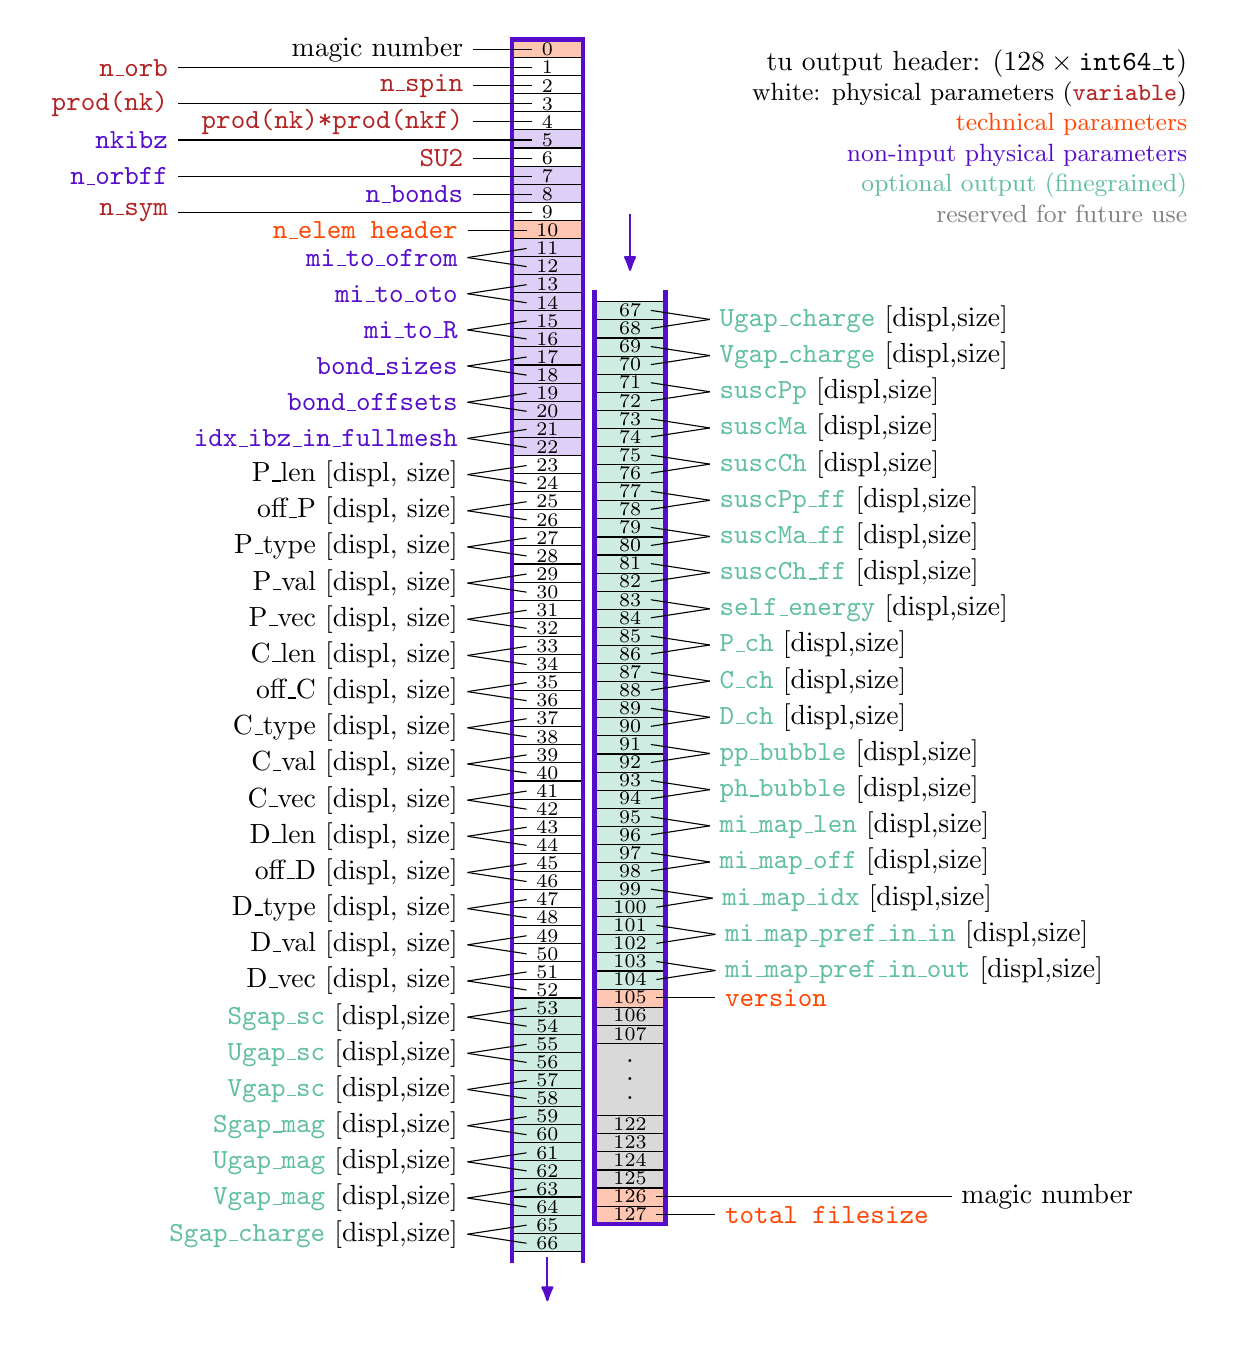
\begin{tikzpicture}[x=5.90552in, y=5.90552in, >={Latex[round]}]
  \clip (0,-0.1) rectangle (1,1.0);
  \tikzmath{
    coordinate \coordA;
    coordinate \coordB;
    int \ibuf;
    real \dbuf;
  }
  \node[anchor=north east] at (0.99,0.99) {\begin{minipage}{3in}%
    \begin{flushright}%
      tu output header: $(128 \times \texttt{int64\_t})$\\
      \small
      white: physical parameters (\tp{variable}) \\
      \textcolor{ForangeRed}{technical parameters} \\
      \textcolor{Fblue}{non-input physical parameters} \\
      \textcolor{Faqua}{optional output (finegrained)} \\
      \textcolor{gray}{reserved for future use}
    \end{flushright}
  \end{minipage}};

  \begin{scope}[shift={(0.41,0.01)}, yscale=0.98, xscale=0.06]
    \colorizeBox{0}{1}{ForangeRed!30!white}
    \colorizeBox{10}{11}{ForangeRed!30!white}  
    
    \colorizeBox{5}{6}{Fblue!20!white}
    \colorizeBox{7}{9}{Fblue!20!white}
    \colorizeBox{11}{23}{Fblue!20!white}

    \colorizeBox{53}{67}{Faqua!30!white}
    \foreach \idx in {1,2,...,67} {
      \tikzmath{
        \dbuf = 1./64.;
        \ibuf = \idx-1;
        \coordA = (0,1-\idx/64.0);
        \coordB = (1,1-\idx/64.0);
      }
      \draw (\coordA) -- node[midway, above, yshift=-0.29em] (cell\ibuf) {\scriptsize\ibuf} (\coordB);
    }
    \tikzmath{ \dbuf = -0.01 - 3./64.; }
    \draw[Fblue, ultra thick] (0,\dbuf) -- (0,1) -- (1,1) -- (1,\dbuf);
    \tikzmath{ \dbuf = -0.005 - 3./64; }
    \draw[Fblue, ->, thick] (0.5,\dbuf) -- (0.5,-0.09);
  \end{scope}
  \begin{scope}[shift={(0.48,-0.059)}, yscale=0.98, xscale=0.06]
    \EcolorizeBox{67}{105}{Faqua!30!white}
    \EcolorizeBox{105}{106}{ForangeRed!30!white}   
    \EcolorizeBox{116}{118}{ForangeRed!30!white}   
    \EcolorizeBox{106}{116}{gray!30!white}   

    \foreach \idx in {0,1,...,40} {
      \tikzmath{
        \dbuf = 1./64.;
        \ibuf = \idx+67;
        \coordA = (0,0.84375-\idx/64.0);
        \coordB = (1,0.84375-\idx/64.0);
      }
      \draw (\coordA) -- node[midway, below, yshift=0.27em] (Ecell\ibuf) {\scriptsize\ibuf} (\coordB);
    }
    \draw (0,0.84375-41.0/64.0) -- (1.0,0.84375-41.0/64.0);
    
    \node[] (q0) at (0.5,0.84375-42.0/64.0) {.};
    \node[] (q1) at (0.5,0.84375-43.0/64.0) {.};
    \node[] (q2) at (0.5,0.84375-44.0/64.0) {.};
    
    \foreach \idx in {0,1,...,5} {
      \tikzmath{
        \dbuf = 1./64.;
        \ibuf = \idx+122;
        \coordA = (0,0.84375-45/64.0-\idx/64.0);
        \coordB = (1,0.84375-45/64.0-\idx/64.0);
      }
      \draw (\coordA) -- node[midway, below, yshift=0.27em] (Ecell\ibuf) {\scriptsize\ibuf} (\coordB);
    }
    \tikzmath{\dbuf = 1.0 - 61.0/64.0;}
    \draw[Fblue, ultra thick] (0,0.85375) -- (0,\dbuf) -- (1,\dbuf) -- (1,0.85375);
    \draw[Fblue, ->, thick] (0.5,0.95-0.03) -- (0.5,0.9005-0.03);
  \end{scope}
  
  \begin{scope}[anchor=east]
    \bracketOne{0}{magic number}
    \draw (cell1.west) -- ++(-0.3,0.0) node {\tp{n\_orb}};
    \draw (cell2.west) -- ++(-0.05,0.0) node {\tp{n\_spin}};
    \draw (cell3.west) -- ++(-0.3,0.0) node {\tp{prod(nk)}};
    \draw (cell4.west) -- ++(-0.05,0.0) node {\tp{prod(nk)*prod(nkf)}};
    \draw (cell5.west) -- ++(-0.3,0.0) node {\nipp{nkibz}};
    \draw (cell6.west) -- ++(-0.05,0.0) node {\tp{SU2}};
    \draw (cell7.west) -- ++(-0.3,0.0) node {\nipp{n\_orbff}};
    \draw (cell8.west) -- ++(-0.05,0.0) node {\nipp{n\_bonds}};
    \draw (cell9.west) -- ++(-0.3,0.0) node {\tp{n\_sym}};
    
    
    \bracketOne{10}{\xp{n\_elem header}}
    
    \bracketTwo{11}{12}{\nipp{mi\_to\_ofrom}}
    \bracketTwo{13}{14}{\nipp{mi\_to\_oto}}
    \bracketTwo{15}{16}{\nipp{mi\_to\_R}}
    \bracketTwo{17}{18}{\nipp{bond\_sizes}}
    \bracketTwo{19}{20}{\nipp{bond\_offsets}}
    \bracketTwo{21}{22}{\nipp{idx\_ibz\_in\_fullmesh}}


    \bracketTwo{23}{24}{\ipd{P\_len}}
    \bracketTwo{25}{26}{\ipd{off\_P}}
    \bracketTwo{27}{28}{\ipd{P\_type}}
    \bracketTwo{29}{30}{\ipd{P\_val}}
    \bracketTwo{31}{32}{\ipd{P\_vec}}
    
    \bracketTwo{33}{34}{\ipd{C\_len}}
    \bracketTwo{35}{36}{\ipd{off\_C}}
    \bracketTwo{37}{38}{\ipd{C\_type}}
    \bracketTwo{39}{40}{\ipd{C\_val}}
    \bracketTwo{41}{42}{\ipd{C\_vec}}
    
    \bracketTwo{43}{44}{\ipd{D\_len}}
    \bracketTwo{45}{46}{\ipd{off\_D}}
    \bracketTwo{47}{48}{\ipd{D\_type}}
    \bracketTwo{49}{50}{\ipd{D\_val}}
    \bracketTwo{51}{52}{\ipd{D\_vec}}
    
   
    \bracketTwo{53}{54}{\oop{Sgap\_sc}}
    \bracketTwo{55}{56}{\oop{Ugap\_sc}}
    \bracketTwo{57}{58}{\oop{Vgap\_sc}}
    
    \bracketTwo{59}{60}{\oop{Sgap\_mag}}
    \bracketTwo{61}{62}{\oop{Ugap\_mag}}
    \bracketTwo{63}{64}{\oop{Vgap\_mag}}
    
    \bracketTwo{65}{66}{\oop{Sgap\_charge}}
    \EbracketTwo{67}{68}{\oop{Ugap\_charge}}
    \EbracketTwo{69}{70}{\oop{Vgap\_charge}}
    
    
    \EbracketTwo{71}{72}{\oop{suscPp}}
    \EbracketTwo{73}{74}{\oop{suscMa}}
    \EbracketTwo{75}{76}{\oop{suscCh}}
    
    \EbracketTwo{77}{78}{\oop{suscPp\_ff}}
    \EbracketTwo{79}{80}{\oop{suscMa\_ff}}
    \EbracketTwo{81}{82}{\oop{suscCh\_ff}}
    
    \EbracketTwo{83}{84}{\oop{self\_energy}}
    
    
    \EbracketTwo{85}{86}{\oop{P\_ch}}
    \EbracketTwo{87}{88}{\oop{C\_ch}}
    \EbracketTwo{89}{90}{\oop{D\_ch}}
    \EbracketTwo{91}{92}{\oop{pp\_bubble}}
    \EbracketTwo{93}{94}{\oop{ph\_bubble}}
    
    
    \EbracketTwo{95}{96}{\oop{mi\_map\_len}}
    \EbracketTwo{97}{98}{\oop{mi\_map\_off}}
    \EbracketTwo{99}{100}{\oop{mi\_map\_idx}}
    \EbracketTwo{101}{102}{\oop{mi\_map\_pref\_in\_in}}
    \EbracketTwo{103}{104}{\oop{mi\_map\_pref\_in\_out}}
    \EbracketOne{105}{\xp{version}}

    \draw (Ecell126.east) -- ++(0.25,0.0) node[anchor=west] {magic number};
    \EbracketOne{127}{\xp{total filesize}}

    \tikzmath{\coordA = 0.5*(Ecell67.east) + 0.5*(Ecell79.east) + (0.1,0.0);
              \coordB = 0.5*(Ecell94.east) + 0.5*(Ecell99.east) + (0.1,0.0);}
  \end{scope}
\end{tikzpicture}
\end{document}

